\section{Parallel reduction operations using OpenMP \punkte{20}}

\subsection*{Dot product}

I compiled \texttt{Skeleton\_codes/dotProduct/dotProduct.cpp} with \texttt{g++ -fopenmp} for each \\ $N \in \{10^5,10^6,10^7,10^8\}$ and ran both OpenMP variants.

\lstinputlisting[
    caption={Reduction-based OpenMP dot product},
    captionpos=b,
    label={lst:dotprod_reduction},
    language=C++,
    numbers=left,
    linerange={57-67},
    firstnumber=57
]{../Skeleton_codes/dotProduct/dotProduct.cpp}

Listing~\ref{lst:dotprod_reduction} lets OpenMP handle partial sums via the \texttt{reduction} clause, avoiding explicit synchronisation while the alternative keeps thread-local buffers and merges them inside a \texttt{critical} region, shown in Listing~\ref{lst:dotprod_critical}.

\lstinputlisting[
    caption={Critical-based OpenMP dot product},
    captionpos=b,
    label={lst:dotprod_critical},
    language=C++,
    numbers=left,
    linerange={69-84},
    firstnumber=69
]{../Skeleton_codes/dotProduct/dotProduct.cpp}

Figures~\ref{fig:dotprod_n1e5}--\ref{fig:dotprod_n1e8} illustrate that even the smallest vector size ($N = 10^5$) benefits from parallel execution: using two threads reduces the runtime from $11.7\,\mathrm{ms}$ to $6.2\,\mathrm{ms}$, while eight threads bring it down further to $2.4\,\mathrm{ms}$. The efficiency plot in Figure~\ref{fig:dotprod_eff} reveals how OpenMP overhead increases with the number of threads. Efficiency, defined as $E = T_1 /(p \cdot T_p)$, decreases whenever speedup grows sub-linearly; for example, a speedup of about 2 on two threads corresponds to $E \approx 1$, whereas a speedup of approximately 4.9 on eight threads results in $E \approx 0.6$. Beyond eight threads, the serial fraction and the cost of \texttt{critical} sections dominate, causing efficiencies to drop below 0.3, although the absolute runtime continues to improve (e.g., $T_{16} = 0.54\,\mathrm{s}$ for $N = 10^7$). The reduction-based variant consistently achieves 5–10\% higher efficiency because it avoids serialized updates. Overall, multithreading is advantageous when the number of threads remains moderate (up to eight) to limit overhead for smaller vectors; for $N \ge 10^7$, the reduction variant scales well up to sixteen threads.

\begin{figure}[H]
    \centering
    \begin{subfigure}{0.45\textwidth}
        \centering
        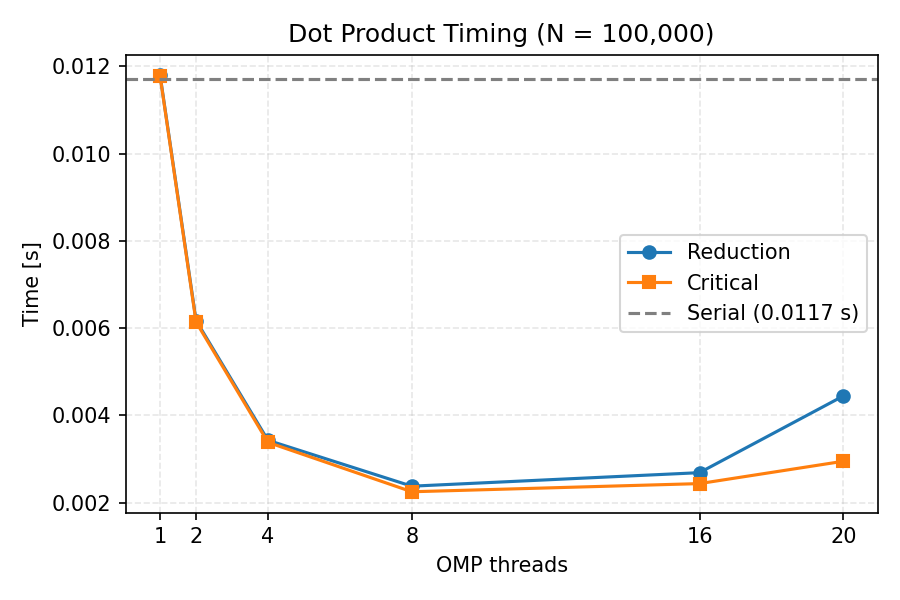
\includegraphics[width=\linewidth]{../Skeleton_codes/dotProduct/plots/dotprod_N100000.png}
        \caption{$N = 10^5$}
        \label{fig:dotprod_n1e5}
    \end{subfigure}
    \hfill
    \begin{subfigure}{0.45\textwidth}
        \centering
        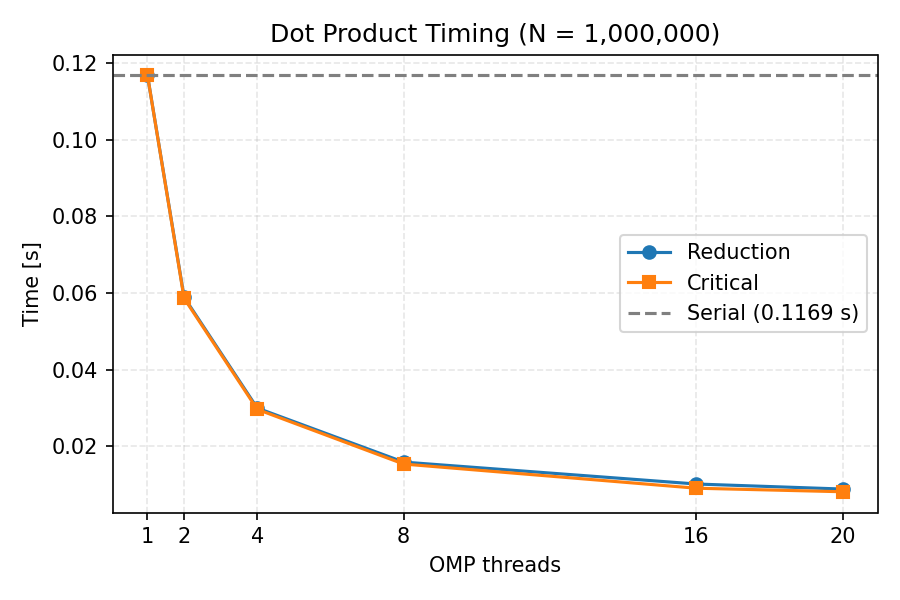
\includegraphics[width=\linewidth]{../Skeleton_codes/dotProduct/plots/dotprod_N1000000.png}
        \caption{$N = 10^6$}
        \label{fig:dotprod_n1e6}
    \end{subfigure}

    \vspace{1em}

    \begin{subfigure}{0.45\textwidth}
        \centering
        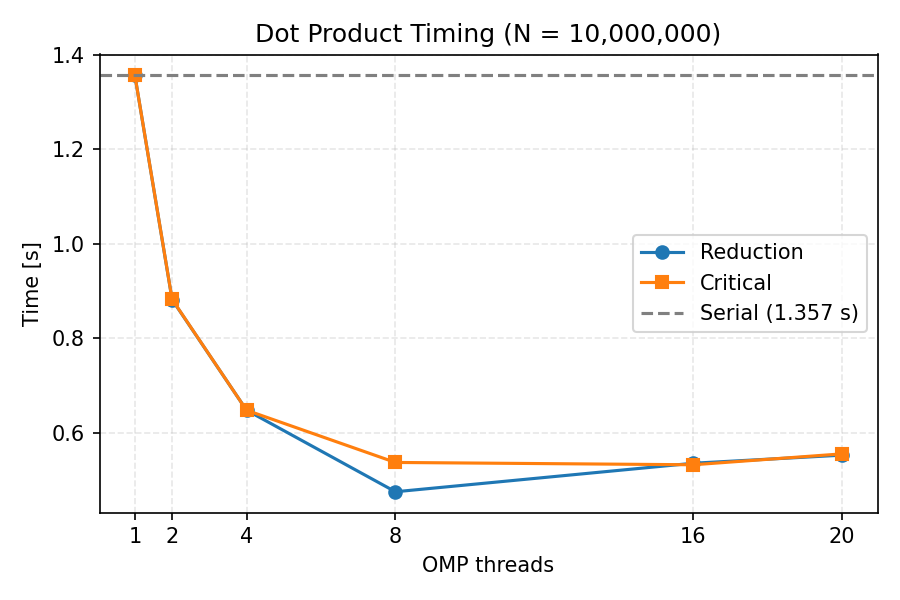
\includegraphics[width=\linewidth]{../Skeleton_codes/dotProduct/plots/dotprod_N10000000.png}
        \caption{$N = 10^7$}
        \label{fig:dotprod_n1e7}
    \end{subfigure}
    \hfill
    \begin{subfigure}{0.45\textwidth}
        \centering
        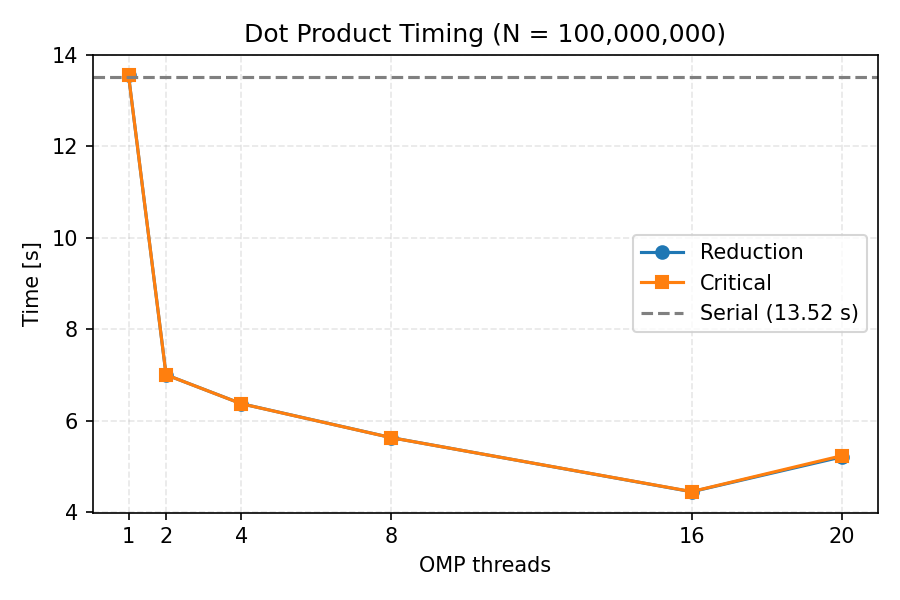
\includegraphics[width=\linewidth]{../Skeleton_codes/dotProduct/plots/dotprod_N100000000.png}
        \caption{$N = 10^8$}
        \label{fig:dotprod_n1e8}
    \end{subfigure}
    \caption{Execution time vs. threads for different vector sizes.}
\end{figure}

\begin{figure}[H]
    \centering
    \IfFileExists{../Skeleton_codes/dotProduct/plots/dotprod_efficiency.png}{
        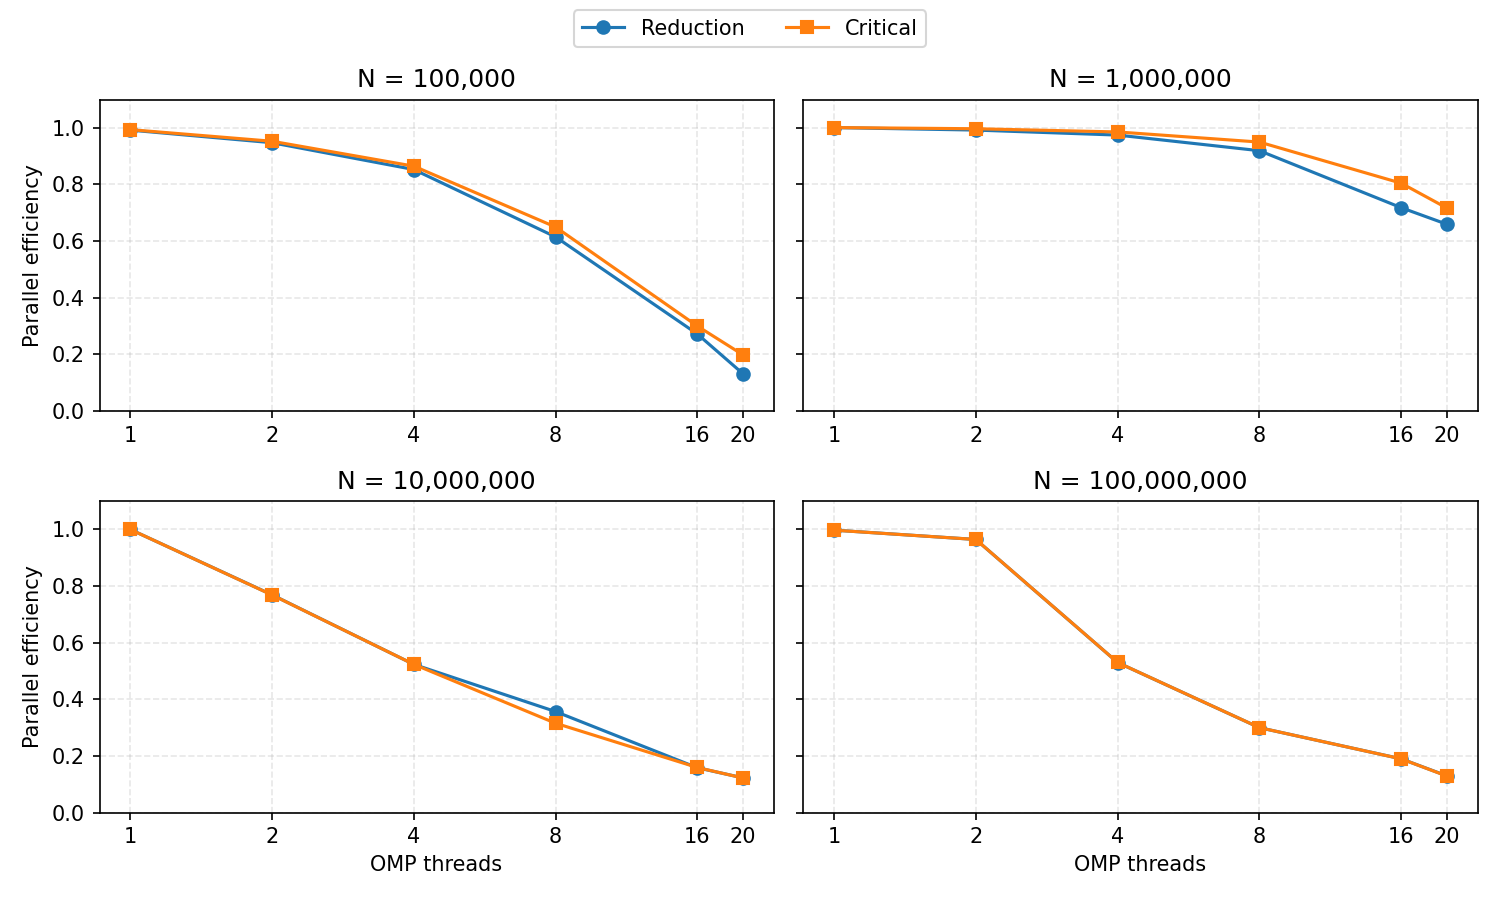
\includegraphics[width=0.75\linewidth]{../Skeleton_codes/dotProduct/plots/dotprod_efficiency.png}
    }{\fbox{Generate \texttt{dotprod\_efficiency.png} via \texttt{plot\_results.py}}}
    \caption{Parallel efficiency $E = T_1 / (p \cdot T_p)$ for the two OpenMP variants.}
    \label{fig:dotprod_eff}
\end{figure}

\newpage

\subsection*{Approximating $\pi$}

I keep $N = 10^{10}$ as mandated. The serial loop in Listing~\ref{lst:pi_serial} walks through all indices with a single accumulator, while the OpenMP variant in Listing~\ref{lst:pi_parallel} retains the same structure but distributes iterations across threads using a reduction clause.

\lstinputlisting[
    caption={Serial midpoint integration for $\pi$},
    captionpos=b,
    label={lst:pi_serial},
    language=C++,
    numbers=left,
    linerange={18-25},
    firstnumber=18
]{../Skeleton_codes/pi/pi.cpp}

\lstinputlisting[
    caption={Parallel midpoint integration with OpenMP reduction},
    captionpos=b,
    label={lst:pi_parallel},
    language=C++,
    numbers=left,
    linerange={29-37},
    firstnumber=29
]{../Skeleton_codes/pi/pi.cpp}

The \texttt{reduction(+:\,sum)} clause is the natural choice here: it is an embarrassingly parallel loop, so each thread can integrate its chunk independently and OpenMP combines the private partial integrals at the end. This avoids serial bottlenecks (e.g., critical sections) and preserves the numerical result for the fixed $N = 10^{10}$.

\begin{figure}[H]
    \IfFileExists{../Skeleton_codes/pi/plots/pi_speedup.csv}{
        \begin{subfigure}{0.45\textwidth}
            \centering
            \csvautotabular{../Skeleton_codes/pi/plots/pi_speedup.csv}
        \end{subfigure}
    }{\fbox{Generate \texttt{pi\_speedup.csv} via \texttt{plot\_speedup\_pi.py}}}
    \hfill
    \IfFileExists{../Skeleton_codes/pi/plots/pi_speedup.png}{
        \begin{subfigure}{0.45\textwidth}
            \centering
            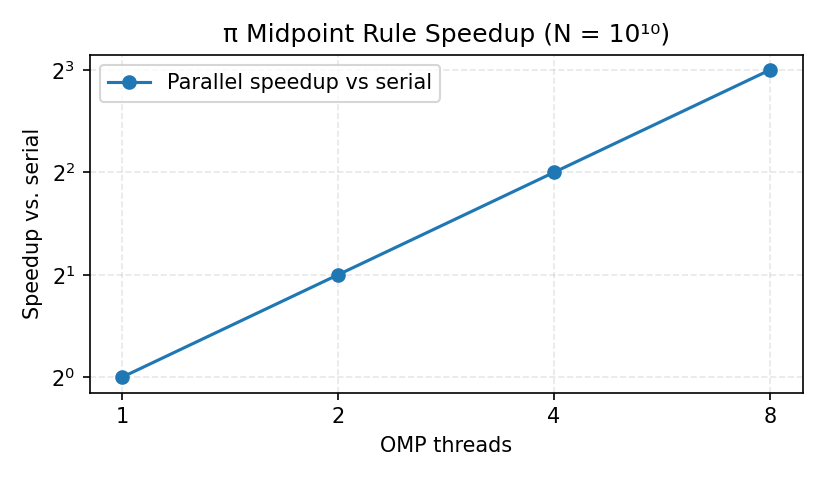
\includegraphics[width=\linewidth]{../Skeleton_codes/pi/plots/pi_speedup.png}
            \vspace{-7em}
        \end{subfigure}
    }{\fbox{Generate \texttt{pi\_speedup.png} via \texttt{plot\_speedup\_pi.py}}}
    \vspace{2em}
    \caption{Timings and speedup for the midpoint $\pi$ approximation with $N = 10^{10}$ (left) parallel speedup vs. serial baseline (right).}
    \label{fig:pi_speedup}
\end{figure}

The speedup, defined as $S_p = T_1/T_p$, measures how much faster the fixed workload executes as the number of threads increases. As shown in Table~\ref{fig:pi_speedup}, every time the number of threads doubles, the runtime is nearly halved, indicating excellent strong scaling. Consequently, the parallel efficiency $E_p = S_p/p$ remains close to one; for example, with eight threads, $E_8 \approx 0.9997$. Since the loop is embarrassingly parallel and the OpenMP reduction clause incurs negligible overhead, the main costs are limited to per-iteration arithmetic and loop control, both of which scale well with increasing thread count. This demonstrates that midpoint integration benefits directly from additional cores without sacrificing accuracy for the prescribed $N = 10^{10}$. An explicit efficiency plot is unnecessary in this case, as the near-ideal speedup already reflects the strong relationship between scaling and efficiency.
